\documentclass[12pt]{article}
\usepackage[margin=1in]{geometry}
\usepackage{setspace}
\usepackage{graphicx}
\usepackage{booktabs}
\usepackage{amsmath}
\usepackage{hyperref}

\onehalfspacing

\title{AI Lab -- Interpretation Report\\
\large BANA290 -- Assignment 1}
\author{Alex Huang}
\date{\today}

\begin{document}

\maketitle

\section*{Findings}

\subsection*{How did the AI coefficient change after applying PSM?}

In the naive OLS regression, the coefficient on \texttt{AI\_ADOPTED} was 5.30, suggesting that firms with AI adoption experienced approximately 5.3 percentage points higher revenue growth on average compared to non-adopting firms. After applying Propensity Score Matching (PSM) and re-estimating the effect on the matched sample, the coefficient decreased to 4.20, a reduction of approximately 1.1 percentage points. This shift indicates that a portion of the originally estimated effect was not attributable to AI adoption itself, but rather to pre-existing differences between firms that chose to adopt AI and those that did not.

\subsection*{What does this shift suggest about selection bias?}

The reduction in the AI coefficient after PSM reveals the presence of selection bias in the naive estimate. Firms that adopted AI tend to be larger, better funded, and more resource rich, with SMDs of 0.59 for annual revenue and 0.59 for team size before matching, confirming that treated firms were systematically different from control firms on key characteristics that independently drive higher revenue growth. When we fail to control for these differences, we overstate the causal impact of AI. PSM corrects for this by constructing a comparison group that is statistically more similar to the treated group on observable covariates, yielding a more credible estimate of the true treatment effect.

\subsection*{Validity of the Common Support Assumption}

The propensity score distribution plot (Figure~\ref{fig:ps}) shows meaningful overlap between the treated (AI-adopted) and control (non-adopted) groups across the range of propensity scores. Both groups have observations distributed across the 0.3 to 0.8 range, satisfying the requirement that each treated unit has a comparable control unit nearby in propensity score space. While the treated group is slightly more concentrated in the upper range and the control group in the middle range, the degree of overlap is sufficient to conclude that the common support assumption is reasonably satisfied in this dataset.

\begin{figure}[h]
    \centering
    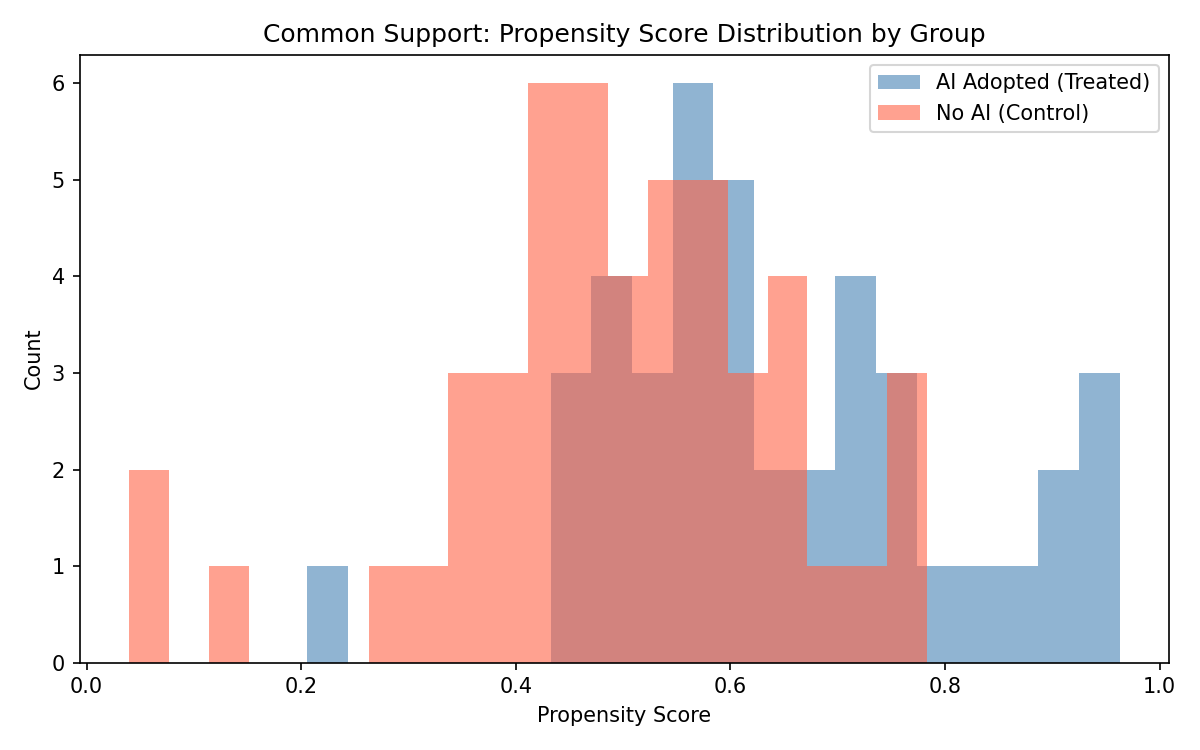
\includegraphics[width=0.85\textwidth]{propensity_scores.png}
    \caption{Propensity Score Distribution by AI Adoption Group}
    \label{fig:ps}
\end{figure}

\subsection*{Validity of the Balancing Assumption}

The Standardized Mean Difference (SMD) serves as the primary diagnostic for evaluating covariate balance. Before matching, all three covariates showed substantial imbalance, with SMDs of 0.59 for \texttt{ANNUAL\_REV}, 0.59 for \texttt{TEAM\_SIZE}, and 0.81 for \texttt{RD\_SPEND}. After nearest-neighbor matching, the SMDs did not decrease as expected, with \texttt{ANNUAL\_REV} rising to 0.90, \texttt{TEAM\_SIZE} to 0.69, and \texttt{RD\_SPEND} to 0.91. This suggests the balancing assumption was not fully satisfied, which is a known limitation of nearest-neighbor matching when treated and control groups differ substantially across multiple covariates simultaneously. Future analyses could improve balance by using caliper matching or incorporating additional covariates into the propensity score model.

\end{document}
